\onehalfspacing
\section{Đề số 24}
\graphicspath{{./img/}}
\begin{bt} 
    Tính hợp lí:
   \begin{enumerate}[a.]
    \item $\frac{7}{-25}+\frac{-18}{25}+\frac{4}{23}+\frac{5}{7}+\frac{19}{23}$
    \item $\frac{7}{19} \cdot \frac{8}{11}+\frac{7}{19} \cdot \frac{3}{11}+\frac{12}{19}$
    \item $(-25) \cdot 125 \cdot 4 \cdot(-8) \cdot(-17)$ 
    \item $\frac{7}{35} \cdot \frac{10}{19}+\frac{7}{35} \cdot \frac{9}{19}-\frac{2}{35}$
   \end{enumerate}
\loigiai{
    \begin{enumerate}
        \item $\frac{7}{-25}+\frac{-18}{25}+\frac{4}{23}+\frac{5}{7}+\frac{19}{23}==\left(\frac{-7}{25}+\frac{-18}{25}\right)+\left(\frac{4}{23}+\frac{19}{23}\right)+\frac{5}{7}=\frac{-25}{25}+\frac{23}{23}+\frac{5}{7}=-1+1+\frac{5}{7}=\frac{5}{7}$
        \item $\frac{7}{19} \cdot \frac{8}{11}+\frac{7}{19} \cdot \frac{3}{11}+\frac{12}{19}==\left(\frac{7}{19} \cdot \frac{8}{11}+\frac{7}{19} \cdot \frac{3}{11}\right)+\frac{12}{19}=\frac{7}{19}\left(\frac{8}{11}+\frac{3}{11}\right)+\frac{12}{19}=\frac{7}{19}+\frac{12}{19}=1$
        \item $(-25) \cdot 125 \cdot 4 \cdot(-8) \cdot(-17)=(-25) \cdot 4 \cdot 125 \cdot(-8) \cdot(-17)$
        $=(-100) \cdot(-1000) \cdot(-17)=-1700000$
        \item $\frac{7}{35} \cdot \frac{10}{19}+\frac{7}{35} \cdot \frac{9}{19}-\frac{2}{35}=\frac{7}{35}\left(\frac{10}{19}+\frac{9}{19}\right)-\frac{2}{35}=\frac{7}{35}-\frac{2}{35}=\frac{5}{35}=\frac{1}{7}$
    \end{enumerate}
}
\end{bt}

\begin{bt}
    Tính giá trị các biểu thức sau:
	\begin{enumerate}[a.]
        \item $A=\frac{1}{2}\left(1+\frac{1}{1.3}\right)\left(1+\frac{1}{2.4}\right)\left(1+\frac{1}{3.5}\right) ... \left(1+\frac{1}{2015.2017}\right)$.
        \item $B=2 x^2-3 x+5$ với $|x|=\frac{1}{2}$.
        \item $C=2 x-2 y+13 x^3 y^2(x-y)+15\left(y^2 x-x^2 y\right)+\left(\frac{2015}{2016}\right)^0$, biết $x-y=0$.
    \end{enumerate}
	\loigiai{
        \begin{enumerate}
            \item $A=\frac{1}{2}\left(1+\frac{1}{1.3}\right)\left(1+\frac{1}{2.4}\right)\left(1+\frac{1}{3.5}\right) \cdot\left(1+\frac{1}{2015.2017}\right)$\\[5px] 
            $=\frac{1}{2}\left(\frac{2}{1} \cdot \frac{2}{3}\right)\left(\frac{3}{2} \cdot \frac{3}{4}\right)\left(\frac{4}{3} \cdot \frac{4}{5}\right) \cdot\left(\frac{2016}{2015} \cdot \frac{2016}{2017}\right) \\[5px]
            =\frac{1}{2}\left(\frac{2}{1} \cdot \frac{2}{3}\right)\left(\frac{3}{2} \cdot \frac{3}{4}\right)\left(\frac{4}{3} \cdot \frac{4}{5}\right) \cdot\left(\frac{2016}{2015} \cdot \frac{2016}{2017}\right)\\[5px]=\frac{2016}{2017}$
            \item Vì $|x|=\frac{1}{2}$ nên $x=\frac{1}{2}$ hoặc $x=-\frac{1}{2}$\\[5px]
            Với $x=\frac{1}{2}$ thì $B=2 \cdot\left(\frac{1}{2}\right)^2-3 \cdot \frac{1}{2}+5=4$\\[5px]
            Với $x=-\frac{1}{2}$ thì $B=2 \cdot\left(-\frac{1}{2}\right)^2-3 \cdot\left(-\frac{1}{2}\right)+5=7$\\[5px]
            Vậy $B=4$ với $x=\frac{1}{2}$ và $B=7$ với $x=-\frac{1}{2}$.
            \item $C=2 x-2 y+13 x^3 y^2(x-y)+15\left(y^2 x-x^2 y\right)+\left(\frac{2015}{2016}\right)^0$\\[5px]
            $=2(x-y)+13 x^3 y^2(x-y)-15 x y(x-y)+1=1(\text { vì } x-y=0)$
        \end{enumerate}
    } 
\end{bt}

\begin{bt}
    \hfill
    \begin{enumerate}[a.]
        \item Tìm $x, y$ biết: $\left(2 x-\frac{1}{6}\right)^2+|3 y+12| \leq 0$.
        \item Tìm $x, y, z$ biết: $\frac{3 x-2 y}{4}=\frac{2 z-4 x}{3}=\frac{4 y-3 z}{2}$ và $x+y+z=18$.
    \end{enumerate}
	\loigiai{
        \begin{enumerate}
            \item Vì $\left(2 x-\frac{1}{6}\right)^2 \geq 0$ với $\forall x ;|3 y+12| \geq 0$ với $\forall y$, do đó:\\[5px]
            $\left(2 x-\frac{1}{6}\right)^2+|3 y+12| \geq 0$ với $\forall x, y$.\\[5px] 
            Theo đề bài thì $\left(2 x-\frac{1}{6}\right)^2+|3 y+12| \leq 0$. Từ đó suy ra:\\[5px]
            $\left(2 x-\frac{1}{6}\right)^2+|3 y+12|=0 \quad$\\[5px] Khi đó $2 x-\frac{1}{6}=0$ và $3 y+12=0\\[5px] \Leftrightarrow x=\frac{1}{12}$ và $y=-4$. Vậy $x=\frac{1}{12}$ và $y=-4$.
            \item Ta có: $\frac{3 x-2 y}{4}=\frac{2 z-4 x}{3}=\frac{4 y-3 z}{2}$ .\\[5px] 
            Suy ra:\\[5px]
            $\frac{4(3 x-2 y)}{16}=\frac{3(2 z-4 x)}{9}=\frac{2(4 y-3 z)}{4}=\frac{12 x-8 y+6 z-12 x+8 y-6 z}{29}=0$\\[5px]
            Do đó: $\frac{3 x-2 y}{4}=0 \Rightarrow 3 x=2 y \Rightarrow \frac{x}{2}=\frac{y}{3}$\\[5px]
            $\frac{2 z-4 x}{3}=0 \Rightarrow 2 z=4 x \Rightarrow \frac{x}{2}=\frac{z}{4}$\\[5px]
            Từ (1) và (2) suy ra $\frac{x}{2}=\frac{y}{3}=\frac{z}{4}$.\\[5px]
            Áp dụng tính chất dãy tỉ số bằng nhau, ta có:\\[5px]
            $\frac{x}{2}=\frac{y}{3}=\frac{z}{4}=\frac{x+y+z}{2+3+4}=\frac{18}{9}=2 .\\[5px] 
            \text { Suy ra: } x=4 ; y=6 ; z=8$
        \end{enumerate}
    }
\end{bt}

\begin{bt}
    \hfill
    \begin{enumerate}[a.]
        \item Tìm các số nguyên $x, y$ biết: $x-2 x y+y-3=0$.
        \item Cho đa thức $\mathrm{f}(x)=x^{10}-101 x^9+101 x^8-101 x^7+\ldots-101 x+101$. Tính $\mathrm{f}(100)$.
    \end{enumerate}
	\loigiai{
        \begin{enumerate}
            \item Ta có: $x-2 x y+y-3=0$
            $\Leftrightarrow 2 x-4 x y+2 y-6=0 \Leftrightarrow 2 x-4 x y+2 y-1=5 \\[5px]
            \Leftrightarrow 2 x(1-2 y)-(1-2 y)=5 \Leftrightarrow(2 x-1)(1-2 y)=5$\\[5px]
            Lập bảng :\\[5px]
            $\begin{array}{|c|c|c|c|c|}
                \hline 2 \mathrm{x}-1 & 1 & 5 & -1 & -5 \\[5px]
                \hline 1-2 \mathrm{y} & 5 & 1 & -5 & -1 \\[5px]
                \hline \mathrm{x} & 1 & 3 & 0 & -2 \\[5px]
                \hline \mathrm{y} & -2 & 0 & 3 & 1 \\[5px]
                \hline & \text { Thỏa mãn } & \text { Thỏa mãn } & \text { Thỏa mãn } & \text { Thỏa mãn } \\[5px]
                \hline
                \end{array}$\\[5px]
            Vậy $(x ; y) \in\{(1 ;-2),(3 ; 0),(0 ; 3),(-2 ; 1)\}$.
            \item Ta có:\\[5px]
                $
                \begin{aligned}
                f(x)= & x^{10}-101 x^9+101 x^8-101 x^7+\ldots-101 x+101 \\[5px]
                & =x^{10}-100 x^9-x^9+100 x^8+x^8-100 x^7-x^7+\ldots-101 x+101 \\[5px]
                & =x^9(x-100)-x^8(x-100)+x^7(x-100)-x^6(x-100)+\ldots+x(x-100)-(x-101)
                \end{aligned}
                $\\[5px]
                Suy ra $f(100)=1$.    
        \end{enumerate}
    }
\end{bt}

\begin{bt}
    Cho tam giác $\mathrm{ABC}$ có ba góc nhọn $(\mathrm{AB}<\mathrm{AC})$. Vẽ về phía ngoài tam giác $\mathrm{ABC}$ các tam giác đều $A B D$ và $A C E$. Gọi $I$ là giao của $C D$ và $B E, K$ là giao của $A B$ và $D C$.
    \begin{enumerate}[a.]
        \item Chứng minh rằng: $\triangle \mathrm{ADC}=\triangle \mathrm{ABE}$.
        \item Chứng minh rằng: $\widehat{\mathrm{DIB}}=60^{\circ}$.
        \item Gọi $\mathrm{M}$ và $\mathrm{N}$ lần lượt là trung điểm của $\mathrm{CD}$ và $\mathrm{BE}$. Chứng minh rằng $\triangle \mathrm{AMN}$ đều.
        \item Chứng minh rằng $IA$ là phân giác của góc $DIE$.
    \end{enumerate}
\loigiai{
    $$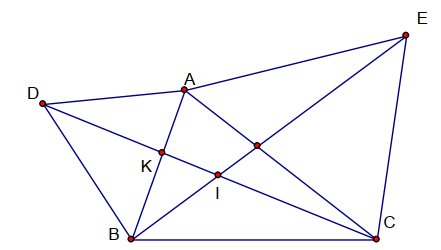
\includegraphics[width=0.5\textwidth]{24-5-lg.png}$$
    \begin{enumerate}
        \item Ta có: $\mathrm{AD}=\mathrm{AB} ; \mathrm{DAC}=\mathrm{BAE}$ và $\mathrm{AC}=\mathrm{AE}$\\[5px]
        Suy ra $\triangle A D C=\triangle A B E$ (c.g.c)
        \item Từ $\triangle \mathrm{ADC}=\triangle \mathrm{ABE}$ (câu a) $\Rightarrow \mathrm{ABE}=\mathrm{ADC}$,
        mà $\mathrm{BKI}=\mathrm{AKD}$ (đối đỉnh).
        Khi đó xét $\triangle \mathrm{BIK}$ và $\triangle \mathrm{DAK}$ suy ra $\mathrm{BIK}=\mathrm{DAK}=60^{\circ}($ (đpcm)
    \end{enumerate}
    $$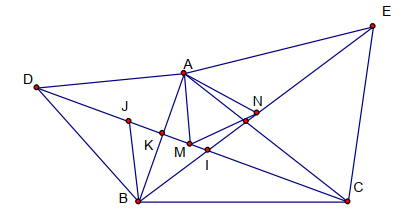
\includegraphics[width=0.5\textwidth]{24-5.1-lg.png}$$
    \begin{enumerate}[c.]
        \item Từ $\triangle \mathrm{ADC}=\triangle \mathrm{ABE}$ (câu a) $\Rightarrow \mathrm{CM}=\mathrm{EN}$ và $\mathrm{ACM}=\mathrm{AEN}$\\[5px]
        $\Rightarrow \triangle \mathrm{ACM}=\Delta \mathrm{AEN}$ (c.g.c) $\Rightarrow \mathrm{AM}=\mathrm{AN}$ và $\mathrm{CAM}=\mathrm{EAN}$\\[5px]
        $\mathrm{MAN}=\mathrm{CAE}=60^{\circ}$. Do đó $\triangle \mathrm{AMN}$ đêu
        \item Trên tia ID lấy điểm $\mathrm{J}$ sao cho $\mathrm{IJ}=\mathrm{IB} \Rightarrow \Delta \mathrm{BIJ}$ đều\\[5px] $\Rightarrow \mathrm{BJ}=\mathrm{BI}$ và $\mathrm{JBI}=\mathrm{DBA}=60^{\circ}$ suy ra $\mathrm{IBA}=\mathrm{JBD}$, kết hợp $\mathrm{BA}=\mathrm{BD}$\\[5px]
        $\Rightarrow \Delta \mathrm{IBA}=\Delta \mathrm{JBD}$ (c.g.c) $\Rightarrow \mathrm{AIB}=\mathrm{DJB}=120^{\circ}$ mà $\mathrm{BID}=60^{\circ}$\\[5px]
        $\Rightarrow \mathrm{DIA}=60^{\circ}$. Từ đó suy ra IA là phân giác của góc DIE
    \end{enumerate}
}
\end{bt}

\begin{bt}
    Cho tam giác $\mathrm{ABC}$ cân tại $\mathrm{A}, A=80^{\circ}$. Ở miền trong tam giác lấy điểm $\mathrm{I}$ sao cho $I B C=10^{\circ}, I C B=30^{\circ}$. Tính $A I B$
\loigiai{
    $$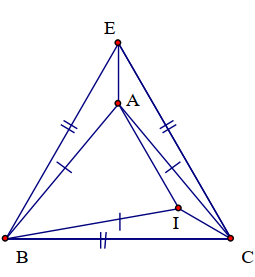
\includegraphics[width=0.4\textwidth]{24-6-lg.png}$$
    Trên nửa mặt phẳng có bờ là đường thẳng $\mathrm{BC}$, chứa điểm $\mathrm{A}$ dựng tam giác đều $\mathrm{BCE}$.\\[5px]
    Vì $\triangle \mathrm{ABC}$ cân tại $\mathrm{A}, A=80^{\circ}$ nên $A B C=A C B=50^{\circ} \Rightarrow A B E=A C E=10^{\circ}$ và điểm $\mathrm{A}$ thuộc miền trong $\triangle$ BCE.\\[5px]
    Dễ dàng chứng minh được\\[5px]
    $\triangle \mathrm{ABE}=\Delta \mathrm{ICB}(\mathrm{g} \cdot \mathrm{c} \cdot \mathrm{g}) \\[5px]
    \Rightarrow \mathrm{BA}=\mathrm{BI} \Rightarrow \Delta \mathrm{ABI} \text { cân tại } \mathrm{B}\\[5px] 
    \text {Ta có }$\\[5px]
    $\mathrm{ABI}=50^{\circ}-10^{\circ}=40^{\circ} \Rightarrow \mathrm{AIB}=\frac{140^{\circ}}{2}=70^{\circ}$
}
\end{bt}

